	\documentclass[12pt,tikz,border=5pt]{standalone}

%	\usepackage[cmyk]{xcolor}

	\usetikzlibrary{mindmap,backgrounds}
	\colorlet{col1}{teal}
	\colorlet{col2}{olive}
	\colorlet{col3}{orange}
	
	\colorlet{partcol0}{col1!80}
	\colorlet{partcol1}{col1!50}
	\colorlet{partcol2}{col1!20}
	
	\begin{document}

%% Part I

	\colorlet{partcol0}{col1!80}
	\colorlet{partcol1}{col1!50}
	\colorlet{partcol2}{col1!20}

	  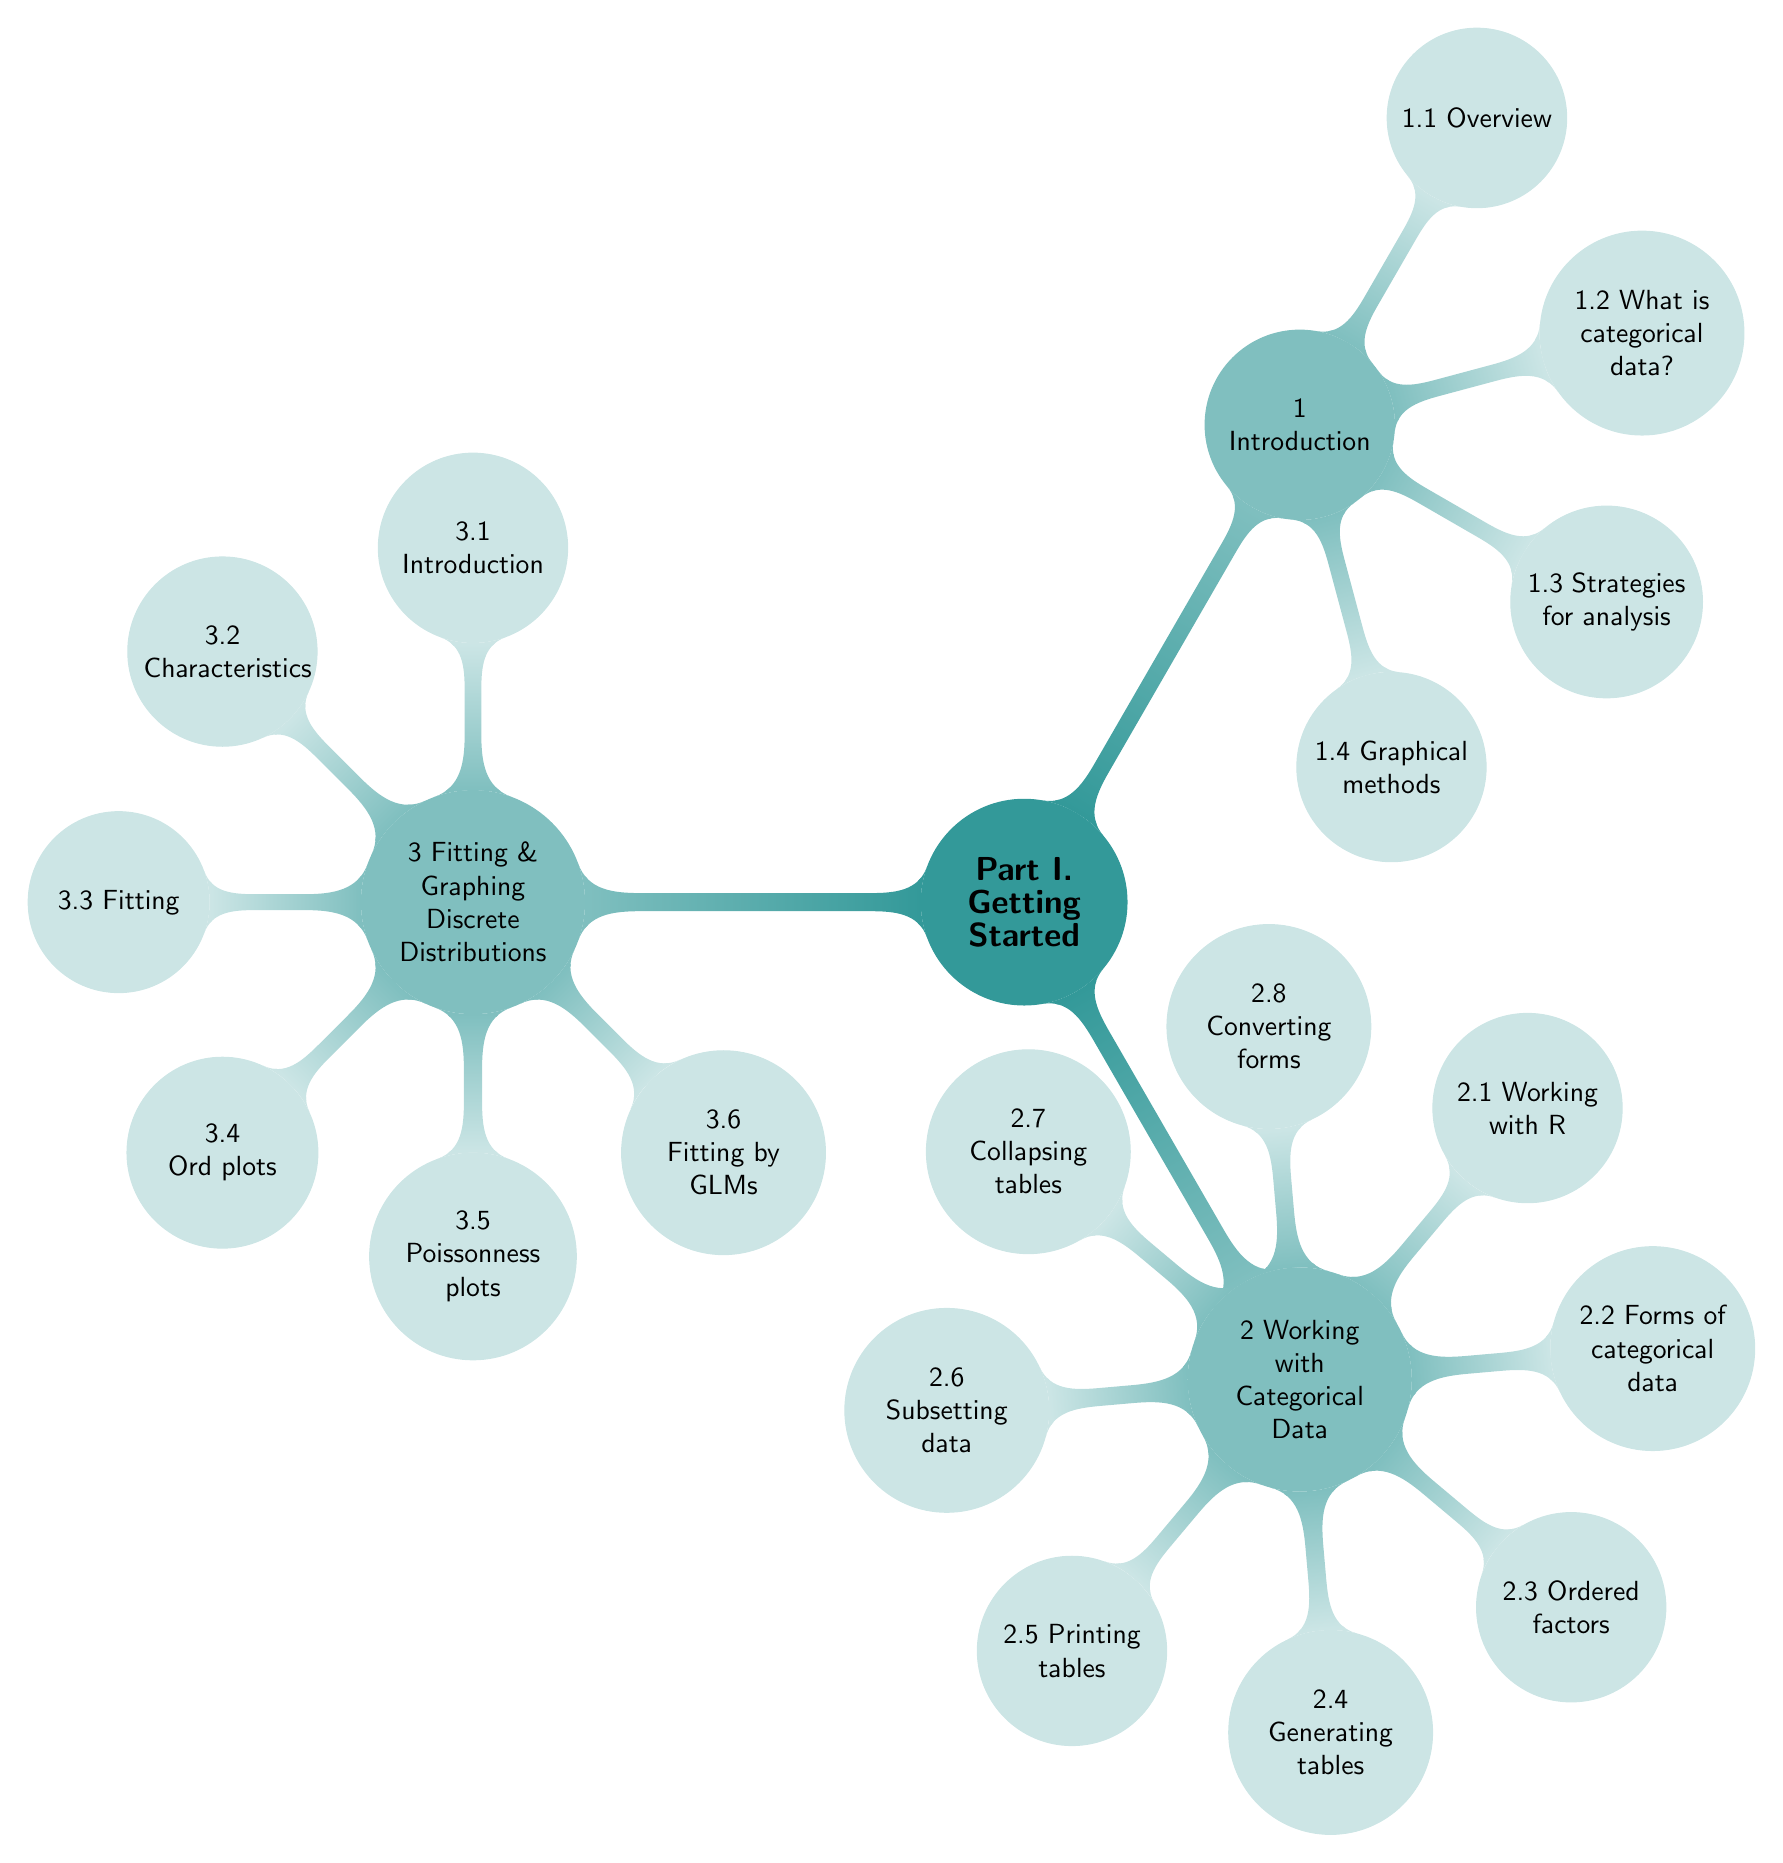
\begin{tikzpicture}[grow cyclic, text width=2cm, align=flush center, every node/.style=concept, concept color=partcol0,
	    level 1/.style={level distance=7cm,sibling angle=120, concept color=partcol1},
	    level 2/.style={level distance=4.5cm,sibling angle=45, concept color=partcol2}]
	    \sffamily
	
		\node {\textbf{\large Part I. Getting Started}} [clockwise from=60]  % root node
			child { node {1 \\ Introduction} [clockwise from=60]
				child { node {1.1 Overview}}
				child { node {1.2 What is categorical data?}}
				child { node {1.3 Strategies for analysis}}
				child { node {1.4 Graphical methods}}
			}
			child { node {2 Working with Categorical Data} [clockwise from=50]
				child { node {2.1 Working with  {R} }} 
				child { node {2.2 Forms of categorical data}}
				child { node {2.3 Ordered factors }}
				child { node {2.4 Generating tables}}
				child { node {2.5 Printing tables}}
				child { node {2.6 Subsetting data}}
				child { node {2.7 Collapsing tables}}
				child { node {2.8 Converting forms}}
	%			child { node {2.9 A complex example}}
			}
			child { node {3 Fitting \& Graphing Discrete Distributions}  [counterclockwise from=90]
				child { node {3.1 \\ Introduction}}
				child { node {3.2 \\ Characteristics}}
				child { node {3.3 Fitting}}
				child { node {3.4 \\ Ord plots}}
				child { node {3.5 \\ Poissonness plots}}
				child { node (sec36) {3.6 \\ Fitting by GLMs}}
		}; % end of part1
	  \end{tikzpicture}

%% Part II
	\colorlet{partcol0}{col2!80}
	\colorlet{partcol1}{col2!50}
	\colorlet{partcol2}{col2!20}

	  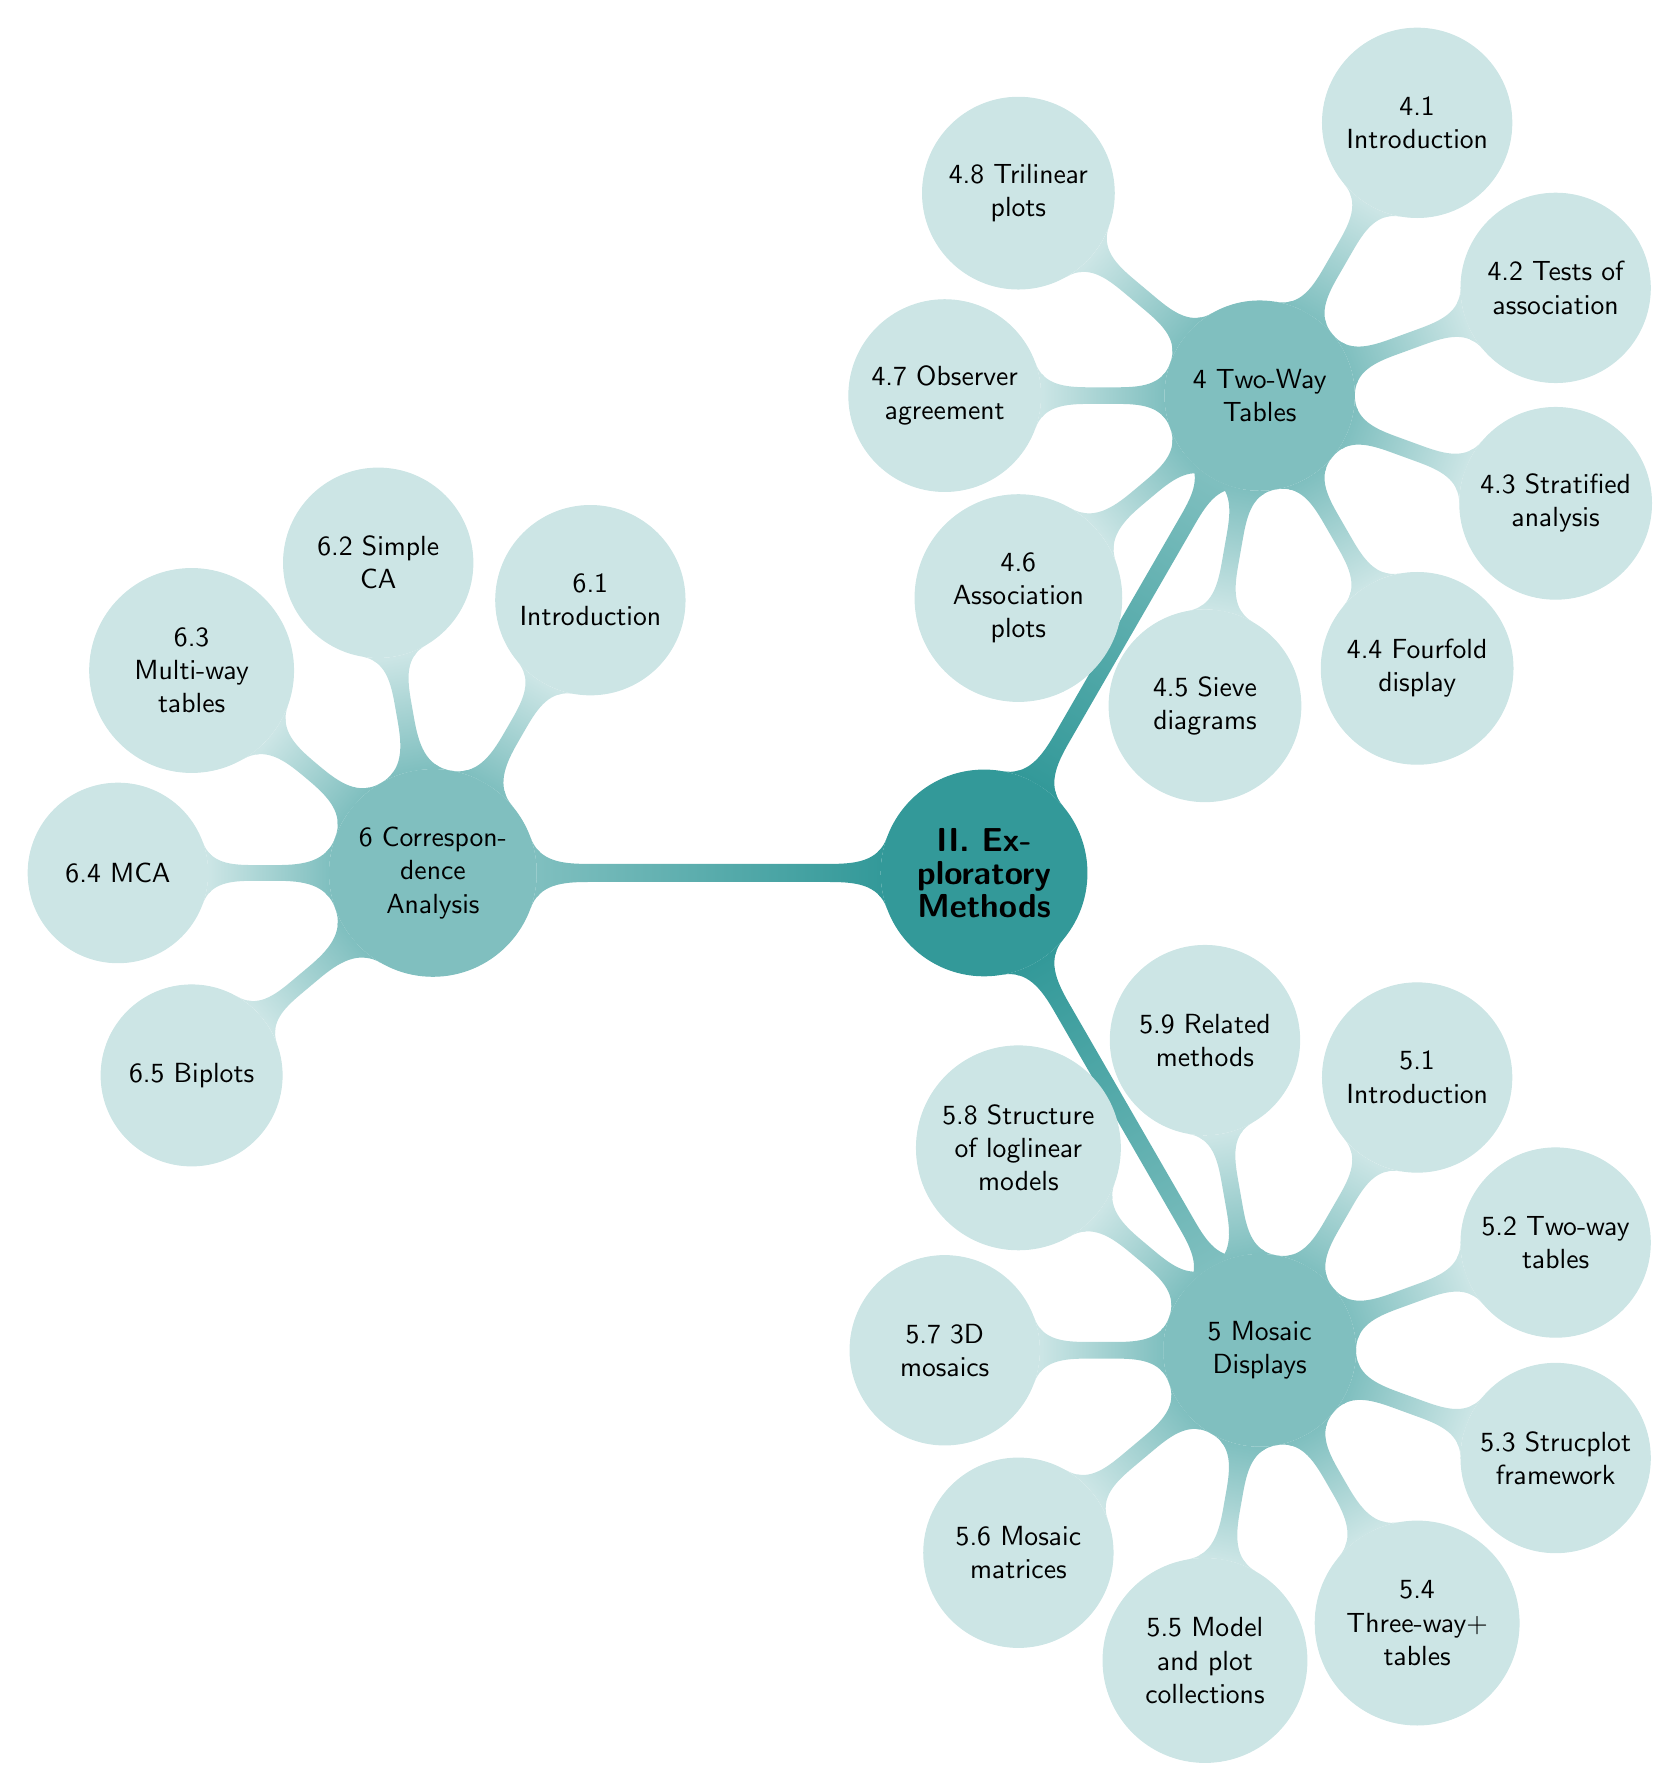
\begin{tikzpicture}[grow cyclic, text width=2cm, align=flush center, every node/.style=concept, concept color=partcol0,
	    level 1/.style={level distance=7cm,sibling angle=120, concept color=partcol1},
	    level 2/.style={level distance=4cm,sibling angle=40, concept color=partcol2}]
	    \sffamily
	
		\node {\textbf{\large II. Exploratory Methods}} [clockwise from=60]  % root node
		child { node {4 Two-Way Tables}
			child { node {4.1 Introduction}}
			child { node {4.2 Tests of association}}
			child { node {4.3 Stratified analysis}}
			child { node {4.4 Fourfold display}}
			child { node {4.5 Sieve diagrams}}
			child { node {4.6 Association plots}}
			child { node {4.7 Observer agreement}}
			child { node {4.8 Trilinear plots}}
		}
		child { node {5 Mosaic Displays}
			child { node {5.1 Introduction}}
			child { node {5.2 Two-way tables}}
			child { node {5.3 Strucplot framework}}
			child { node {5.4 Three-way$+$ tables}}
			child { node {5.5 Model and plot collections}}
			child { node {5.6 Mosaic matrices}}
			child { node {5.7 3D mosaics}}
			child { node {5.8 Structure of loglinear models}}
			child { node {5.9 Related methods}}
		}
		child { node {6 Correspondence Analysis} [counterclockwise from=60]
			child { node {6.1 Introduction}} 
			child { node {6.2 Simple CA}}
			child { node {6.3 Multi-way tables}}
			child { node {6.4 MCA}}
			child { node {6.5 Biplots}}
		}; % end of part2

	  \end{tikzpicture}

%% Part III
	\colorlet{partcol0}{col3!80}
	\colorlet{partcol1}{col3!50}
	\colorlet{partcol2}{col3!20}

	  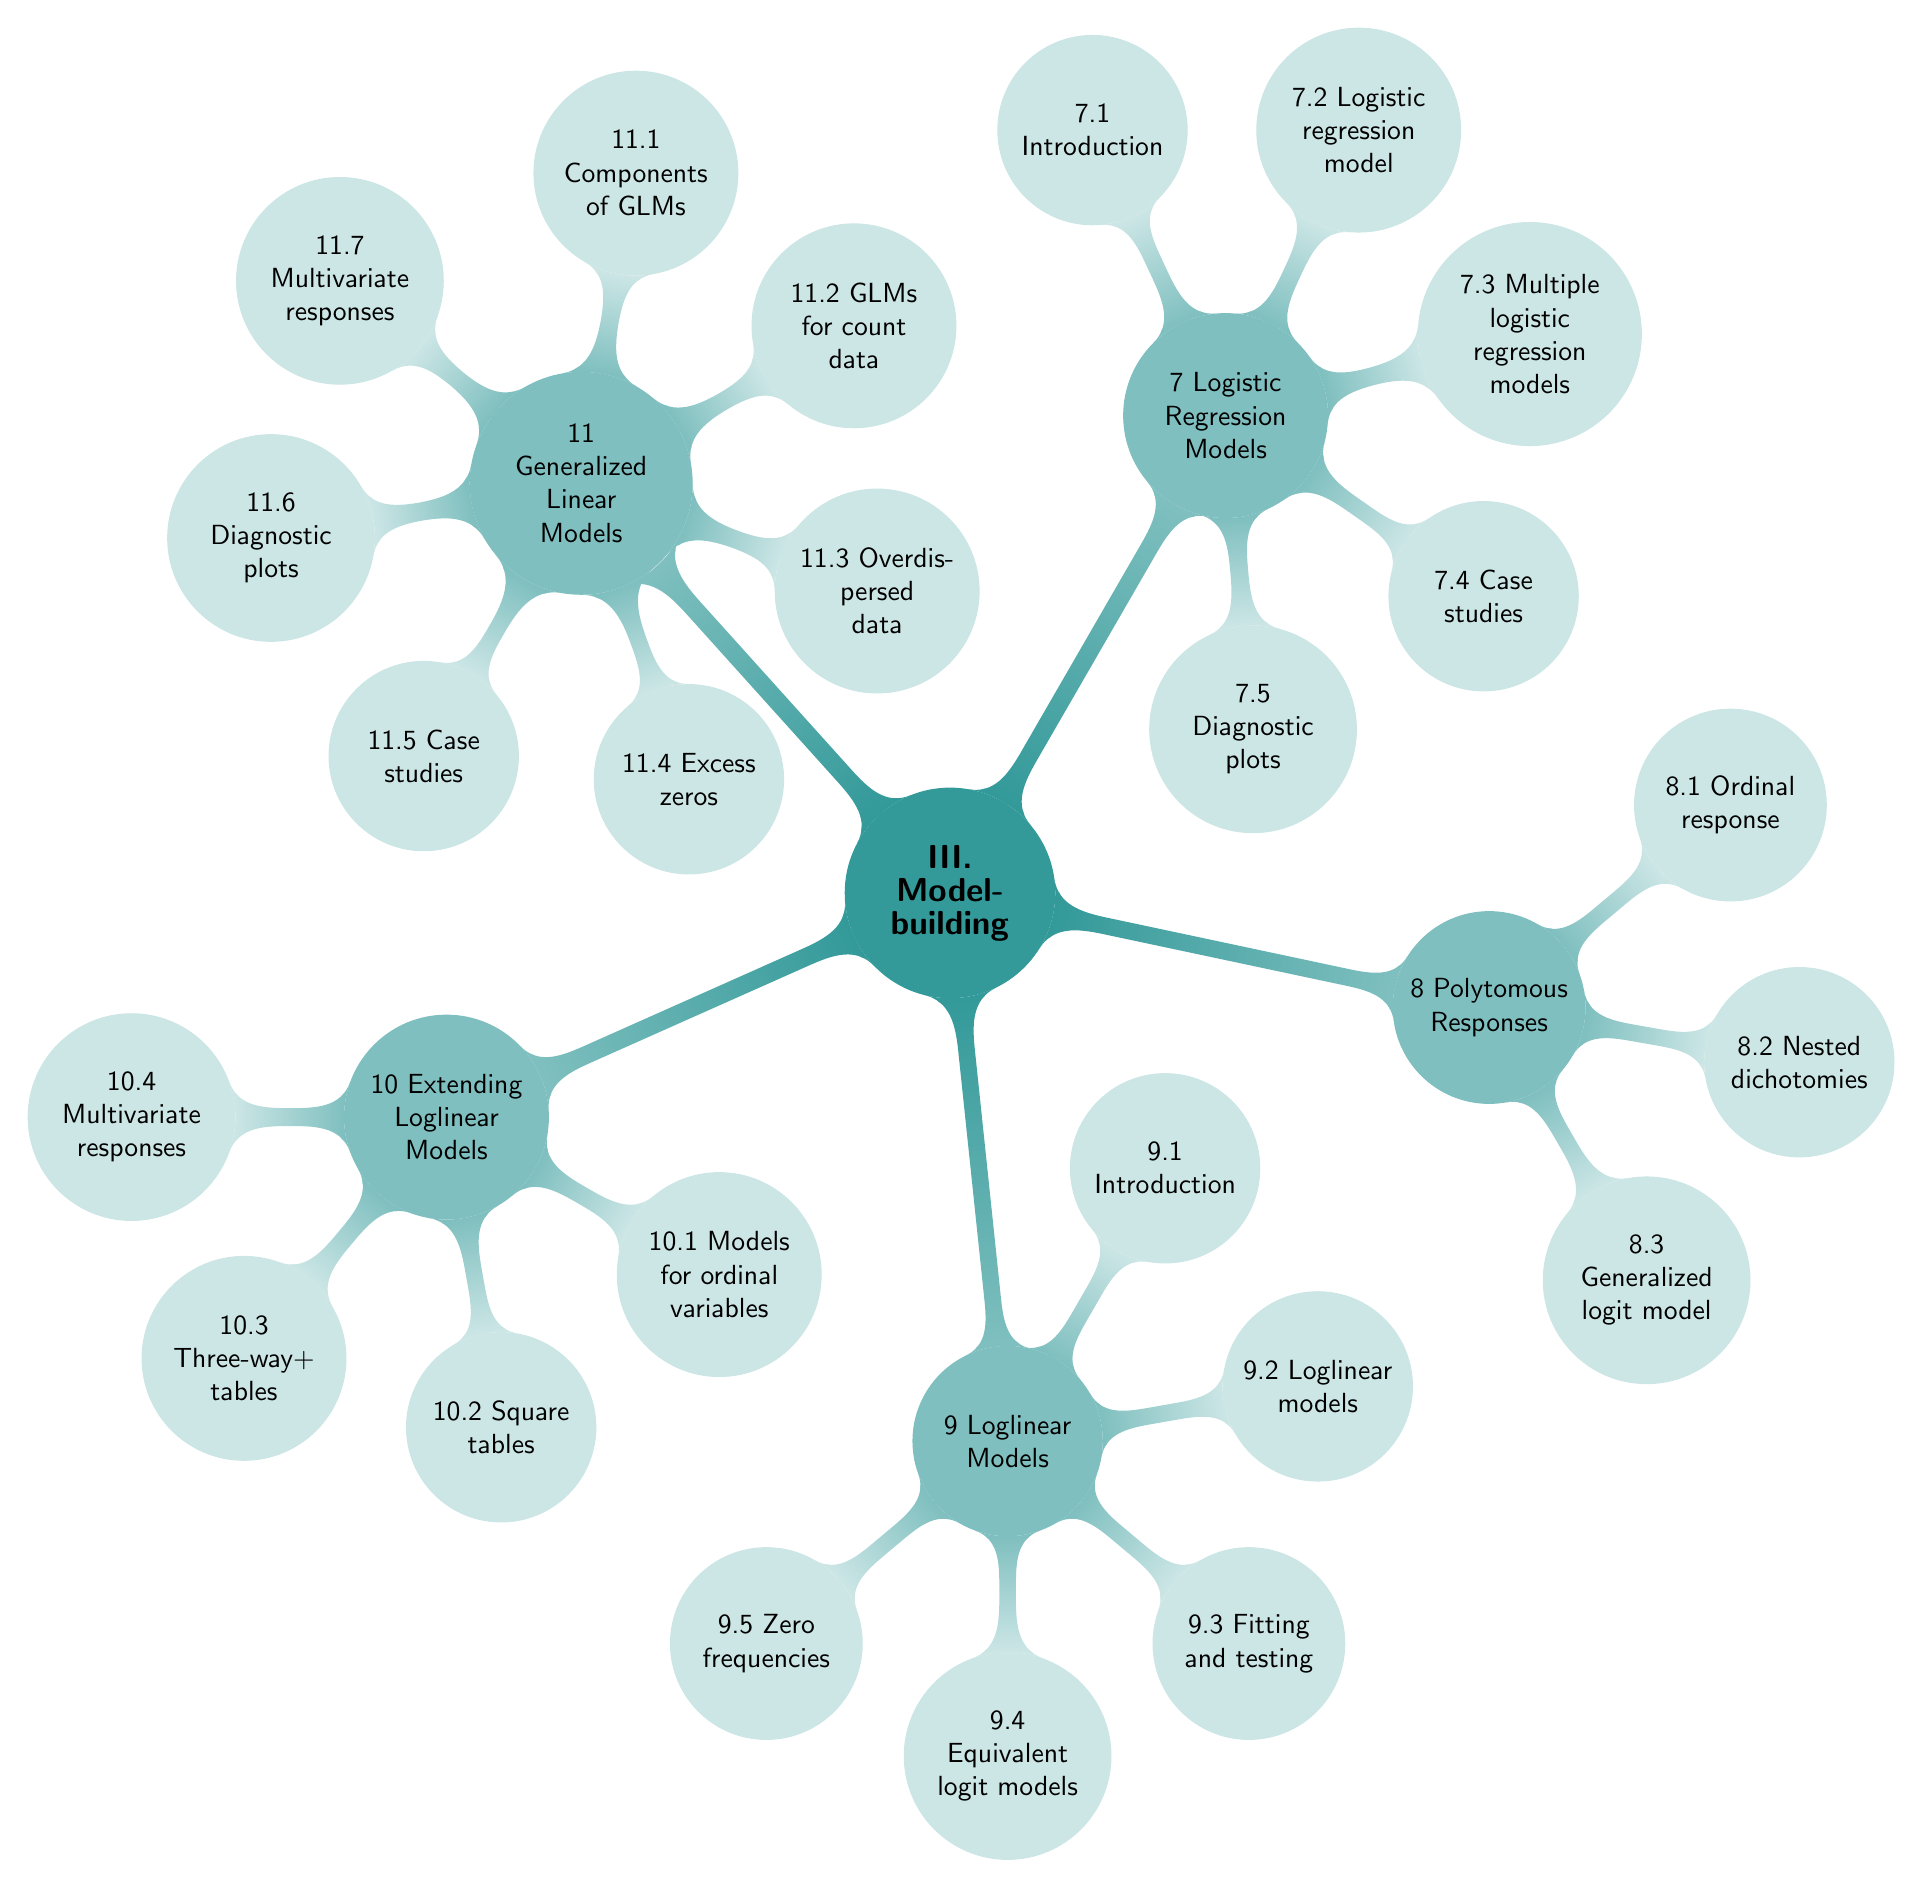
\begin{tikzpicture}[grow cyclic, text width=2cm, align=flush center, every node/.style=concept, concept color=partcol0,
	    level 1/.style={level distance=7cm,sibling angle=72, concept color=partcol1},
	    level 2/.style={level distance=4cm,sibling angle=50, concept color=partcol2}]
	    \sffamily
	
		\node {\textbf{\large III. Model-building}} [clockwise from=60]  % root node
		child { node {7 Logistic Regression Models}  [clockwise from=115]
			child { node {7.1 Introduction}}
			child { node {7.2 Logistic regression model}}
			child { node {7.3 Multiple logistic regression models}}
			child { node {7.4 Case studies}}
			child { node {7.5 Diagnostic plots}}
		}
		child { node {8  Polytomous Responses}  [clockwise from=40]
			child { node {8.1 Ordinal response}}
			child { node {8.2 Nested dichotomies}}
			child { node {8.3 Generalized logit model}}
		}
		child { node {9 Loglinear Models}
			child { node {9.1 Introduction}}
			child { node {9.2 Loglinear models}}
			child { node {9.3 Fitting and testing}}
			child { node {9.4 Equivalent logit models}}
			child { node {9.5 Zero frequencies}}
		}
		child { node {10 Extending Loglinear Models}   [clockwise from=-30]
			child { node {10.1 Models for ordinal variables}}
			child { node {10.2 Square tables}}
			child { node {10.3 Three-way$+$ tables}}
			child { node {10.4 Multivariate responses}}
		}
		child { node {11 Generalized Linear Models}  [clockwise from=80]
			child { node {11.1 Components of GLMs}}
			child { node {11.2 GLMs for count data}}
			child { node {11.3 Overdispersed data}}
			child { node {11.4 Excess zeros}}
			child { node {11.5 Case studies}}
			child { node {11.6 Diagnostic plots}}
			child { node {11.7 Multivariate responses}}
		};
	  \end{tikzpicture}
	\end{document}
